% Figura 1: forma do pulo em L para os dígitos 0, 1 e 2.
%
% Como ler o código: cada L tem (2+d) passos na horizontal e (1+d) na vertical.
% As casas brancas formam o L do dígito 0; as casas coloridas são as d casas
% acrescentadas em cada perna. Para mudar as cores, edite \colorlet abaixo; para mostrar
% mais dígitos, acrescente um par "d/posição" na lista do \foreach (por exemplo 3/17.2).
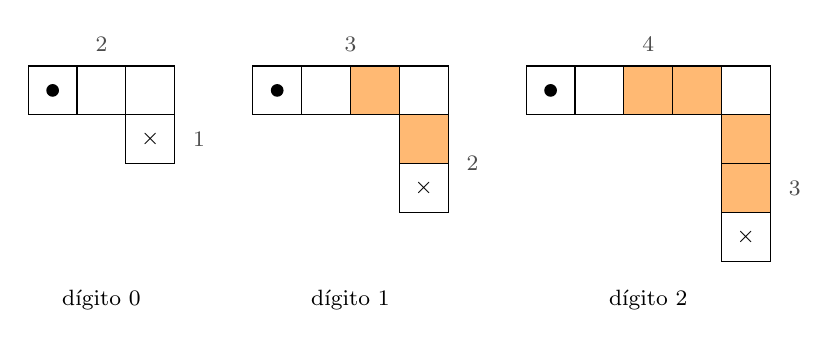
\begin{tikzpicture}[x=0.62cm,y=0.62cm,font=\footnotesize]
  \colorlet{extra}{orange!55}
  \foreach \d/\xo in {0/0, 1/4.6, 2/10.2} {
    \pgfmathtruncatemacro{\pl}{2+\d}   % passos na horizontal = coluna do canto
    \pgfmathtruncatemacro{\pc}{1+\d}   % passos na vertical
    % perna horizontal (linha de cima)
    \foreach \c in {0,...,\pl} {
      \pgfmathtruncatemacro{\ex}{and(\c>=2,\c<\pl)}
      \ifnum\ex=1 \def\cor{extra}\else\def\cor{white}\fi
      \draw[fill=\cor] ({\xo+\c},0) rectangle ++(1,1);
    }
    % perna vertical (abaixo do canto)
    \foreach \r in {1,...,\pc} {
      \pgfmathtruncatemacro{\ex}{\r<=\d}
      \ifnum\ex=1 \def\cor{extra}\else\def\cor{white}\fi
      \draw[fill=\cor] ({\xo+\pl},{-\r}) rectangle ++(1,1);
    }
    % casa de partida (ponto) e casa de chegada (x)
    \fill ({\xo+0.5},0.5) circle (0.13);
    \node at ({\xo+\pl+0.5},{-\pc+0.5}) {$\times$};
    % comprimento de cada perna, em passos
    \node[gray!60!black] at ({\xo+(\pl+1)/2},1.45) {\pl};
    \node[gray!60!black] at ({\xo+\pl+1.5},{-\pc/2}) {\pc};
    % rótulo do dígito
    \node[anchor=north] at ({\xo+(\pl+1)/2},-3.4) {dígito $\d$};
  }
\end{tikzpicture}
